% Required packages: tikz, lmodern
% Required TikZ libraries: none
% Target width: 160 mm maximum
% Minimum text size: 9 pt
% Colour/greyscale intent: colour_and_greyscale; direct symbols and text carry all meaning
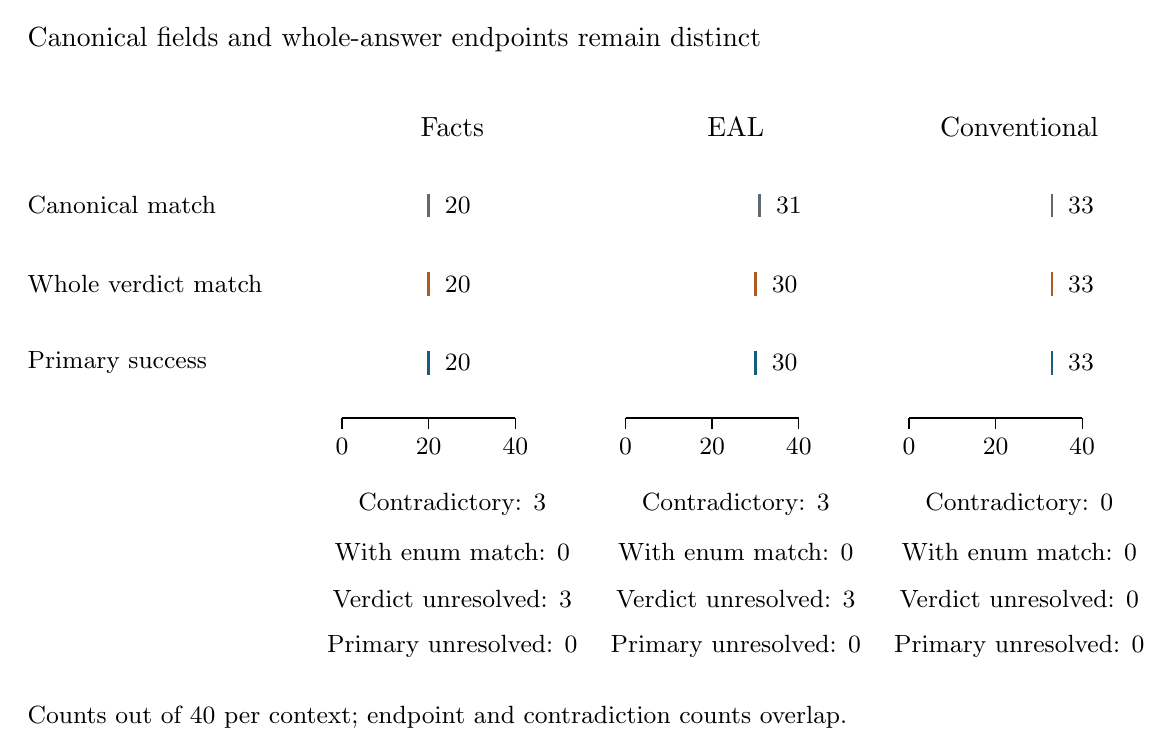
\begin{tikzpicture}[x=1mm,y=1mm,font=\fontsize{9}{11}\selectfont]
\definecolor{successblue}{HTML}{165D81}
\definecolor{failureorange}{HTML}{AD5920}
\definecolor{neutralgrey}{HTML}{616970}
\node[anchor=west,inner sep=0pt,font=\fontsize{10}{12}\selectfont] at (0,74) {Canonical fields and whole-answer endpoints remain distinct};
\node[anchor=west,inner sep=0pt] at (0,53) {Canonical match};
\node[anchor=west,inner sep=0pt] at (0,43) {Whole verdict match};
\node[anchor=west,inner sep=0pt] at (0,33) {Primary success};
\node[inner sep=0pt,font=\fontsize{10}{12}\selectfont] at (54,63) {Facts};
\draw[neutralgrey,line width=1pt] (51.000,51.5) -- (51.000,54.5);
\node[anchor=west,inner sep=0pt] at (53.000,53) {20};
\draw[failureorange,line width=1pt] (51.000,41.5) -- (51.000,44.5);
\node[anchor=west,inner sep=0pt] at (53.000,43) {20};
\draw[successblue,line width=1pt] (51.000,31.5) -- (51.000,34.5);
\node[anchor=west,inner sep=0pt] at (53.000,33) {20};
\draw[black,line width=0.5pt] (40,26) -- (62,26);
\draw[black,line width=0.5pt] (40.000,26) -- (40.000,24.6);\node[anchor=north,inner sep=0pt] at (40.000,23.5) {0};
\draw[black,line width=0.5pt] (51.000,26) -- (51.000,24.6);\node[anchor=north,inner sep=0pt] at (51.000,23.5) {20};
\draw[black,line width=0.5pt] (62.000,26) -- (62.000,24.6);\node[anchor=north,inner sep=0pt] at (62.000,23.5) {40};
\node[inner sep=0pt] at (54,15) {Contradictory: 3};
\node[inner sep=0pt] at (54,9) {With enum match: 0};
\node[inner sep=0pt] at (54,3) {Verdict unresolved: 3};
\node[inner sep=0pt] at (54,-3) {Primary unresolved: 0};
\node[inner sep=0pt,font=\fontsize{10}{12}\selectfont] at (90,63) {EAL};
\draw[neutralgrey,line width=1pt] (93.050,51.5) -- (93.050,54.5);
\node[anchor=west,inner sep=0pt] at (95.050,53) {31};
\draw[failureorange,line width=1pt] (92.500,41.5) -- (92.500,44.5);
\node[anchor=west,inner sep=0pt] at (94.500,43) {30};
\draw[successblue,line width=1pt] (92.500,31.5) -- (92.500,34.5);
\node[anchor=west,inner sep=0pt] at (94.500,33) {30};
\draw[black,line width=0.5pt] (76,26) -- (98,26);
\draw[black,line width=0.5pt] (76.000,26) -- (76.000,24.6);\node[anchor=north,inner sep=0pt] at (76.000,23.5) {0};
\draw[black,line width=0.5pt] (87.000,26) -- (87.000,24.6);\node[anchor=north,inner sep=0pt] at (87.000,23.5) {20};
\draw[black,line width=0.5pt] (98.000,26) -- (98.000,24.6);\node[anchor=north,inner sep=0pt] at (98.000,23.5) {40};
\node[inner sep=0pt] at (90,15) {Contradictory: 3};
\node[inner sep=0pt] at (90,9) {With enum match: 0};
\node[inner sep=0pt] at (90,3) {Verdict unresolved: 3};
\node[inner sep=0pt] at (90,-3) {Primary unresolved: 0};
\node[inner sep=0pt,font=\fontsize{10}{12}\selectfont] at (126,63) {Conventional};
\draw[neutralgrey,line width=1pt] (130.150,51.5) -- (130.150,54.5);
\node[anchor=west,inner sep=0pt] at (132.150,53) {33};
\draw[failureorange,line width=1pt] (130.150,41.5) -- (130.150,44.5);
\node[anchor=west,inner sep=0pt] at (132.150,43) {33};
\draw[successblue,line width=1pt] (130.150,31.5) -- (130.150,34.5);
\node[anchor=west,inner sep=0pt] at (132.150,33) {33};
\draw[black,line width=0.5pt] (112,26) -- (134,26);
\draw[black,line width=0.5pt] (112.000,26) -- (112.000,24.6);\node[anchor=north,inner sep=0pt] at (112.000,23.5) {0};
\draw[black,line width=0.5pt] (123.000,26) -- (123.000,24.6);\node[anchor=north,inner sep=0pt] at (123.000,23.5) {20};
\draw[black,line width=0.5pt] (134.000,26) -- (134.000,24.6);\node[anchor=north,inner sep=0pt] at (134.000,23.5) {40};
\node[inner sep=0pt] at (126,15) {Contradictory: 0};
\node[inner sep=0pt] at (126,9) {With enum match: 0};
\node[inner sep=0pt] at (126,3) {Verdict unresolved: 0};
\node[inner sep=0pt] at (126,-3) {Primary unresolved: 0};
\node[anchor=west,inner sep=0pt] at (0,-12) {Counts out of 40 per context; endpoint and contradiction counts overlap.};
\end{tikzpicture}
